\makeheading{Week 10}{\daterange{2021-11-17}{2021-11-24}}%chktex 8
\section{The Poisson Process}
\subsection*{Counting Process}
\begin{Regular}
    \textbf{Definition}: A \emph{counting process} $ \Set[\big]{N(t),t\ge 0} $ is a stochastic process in which $N(t)$ represents
    the number of events that happen (or occur) by time $t$, where the index $t$ measures time over
    a continuous range.

    Some examples of counting processes $ \Set[\big]{N(t),t\ge 0} $ might include:
    \begin{enumerate}[(1)]
        \item $N(t)$ represents the number of automobile accidents at a specified intersection by week $t$,
        \item $N(t)$ represents the number of births by year $t$ in Canada,
        \item $N(t)$ represents the number of visits to a particular webpage by time $t$,
        \item $N(t)$ represents the number of customers who enter a store by time $t$,
        \item $N(t)$ represents the number of accident claims reported to an insurance company by time
              $t$.
    \end{enumerate}
    \textbf{Basic Properties of Counting Processes}:
    \begin{enumerate}[(1)]
        \item $ N(0)=0 $.
        \item $ N(t) $ is a non-negative integer $ \forall t\ge 0 $ (i.e., $ N(t)\in\mathbb{N}\;\forall t\ge 0 $).
        \item If $ s<t $, then $ N(s)\le N(t) $.
        \item $ N(t)-N(s) $ counts the number of events to occur in the time interval $ (s,t] $ for $ s<t $.
    \end{enumerate}
\end{Regular}
\subsection*{Independent and Stationary Increments}
We now introduce two important properties associated with counting processes.
\begin{Regular}
    \textbf{Definition}: A counting process $ \Set[\big]{N(t),t\ge 0} $ has \emph{independent increments} if $ N(t_1)-N(s_1) $ is
    independent of $ N(t_2)-N(s_2) $ whenever $ (s_1,t_1]\cap (s_2,t_2]=\emptyset $ for all choices of $ s_1,t_1,s_2,t_2 $
    (i.e., the number of events in non-overlapping time intervals are assumed to be independent of each other).
\end{Regular}
\begin{Regular}
    \textbf{Definition}: A counting process $ \Set[\big]{N(t),t\ge 0} $ has \emph{stationary increments} if the distribution
    of the number of events in $ (s,s+t] $ (i.e., $ N(s+t)-N(s) $) depends only on $ t $, the length of the time interval.
    In this case, $ N(s+t)-N(s) $ has the same probability distribution as $ N(0+t)-N(0)=N(t) $, the number of events
    occurring in the interval $ [0,t] $.
\end{Regular}
\underline{Remark}: As the diagram below indicates, the assumption of stationary and independent
increments is essentially equivalent to stating that, at any point in time, the process
$ \Set[\big]{N(t),t\ge 0} $ \emph{probabilistically restarts itself}.
\begin{figure}[!htbp]
    \centering
    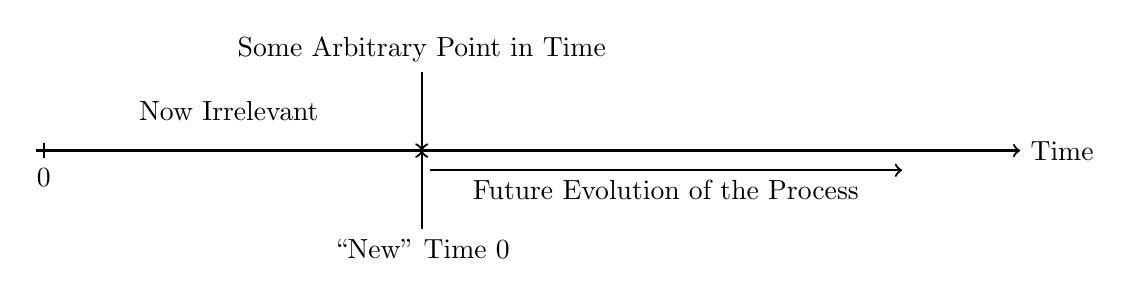
\begin{tikzpicture}[thick]
        % draw horizontal line
        \draw[->] (0,0) -- (12.5,0);
        \draw[-] (0.1,0.1) -- (0.1,-0.1) node[anchor=north] {$0$};
        \node[anchor=west] at (12.5,0) {Time};
        \draw[->] (5,-0.25) -- (11,-0.25) node[anchor=north,midway] {Future Evolution of the Process};
        \draw[<-] (4.9,0) -- (4.9,-1) node[anchor=north] {``New'' Time $0$};
        \draw[<-] (4.9,0) -- (4.9,1) node[anchor=south] {Some Arbitrary Point in Time};
        \draw[draw=none] (0,0.25) -- (4.9,0.25) node[anchor=south,midway] {Now Irrelevant};
    \end{tikzpicture}
\end{figure}
\subsection*{$\order{h}$ Function}
Before introducing the formal definition of a Poisson process, we first introduce a few mathematical tools which are needed.
\begin{Regular}
    \textbf{Definition}: A function $ y=f(x) $ is said to be ``$ \order{h} $'' (i.e., of order $ h $) if
    \[ \lim\limits_{{h} \to {0}}\frac{f(h)}{h}=0. \]
    \tcblower{}
    \underline{Remark}: An $ \order{h} $ function $ y=f(x) $ is one in which $ f(h) $ approaches $ 0 $ faster than $ h $ does.
\end{Regular}
\begin{Example}
    \textbf{Examples}:
    \begin{enumerate}[(1)]
        \item $ y=f(x)=x $. Note that
              \[ \lim\limits_{{h} \to {0}}\frac{f(h)}{h}=\lim\limits_{{h} \to {0}}\frac{h}{h}=\lim\limits_{{h} \to {0}}1\ne 0. \]
              Thus, $ y=x $ is not of order $ h $.
        \item $ y=f(x)=x^2 $. Note that
              \[ \lim\limits_{{h} \to {0}}\frac{f(h)}{h}=\lim\limits_{{h} \to {0}}\frac{h^2}{h}=\lim\limits_{{h} \to {0}}h=0. \]
              Thus, $ y=x^2 $ is of order $ h $. In fact, the function of the form $ y=x^r $ is clearly of order $ h $ provided that $ r>1 $.
    \end{enumerate}
\end{Example}
\begin{enumerate}[(3)]
    \item Suppose that $ \Set[\big]{f_i(x)}_{i=1}^n $ is a sequence of $ \order{h} $ functions. Consider the linear combination of $ \order{h} $
          functions, namely $ y=\sum_{i=1}^{n}c_i f_i(x) $, and note that
          \[ \lim\limits_{{h} \to {0}}\frac{\sum_{i=1}^{n}c_i f_i}{h}=\sum_{i=1}^{n}c_i \underbrace{\lim\limits_{{h} \to {0}}\frac{f_i(h)}{h}}_{=0}=0. \]
          Thus, a linear combination of $ \order{h} $ functions is still of order $ h $.

          \underline{Remark}: In most cases, this result is actually true when $ n=\infty $.
\end{enumerate}
\subsection*{Poisson Process}
\begin{Regular}
    \textbf{Definition}: A counting process $ \Set[\big]{N(t),t\ge 0} $ is said to be a \emph{Poisson process} at rate $ \lambda $
    if the following three conditions hold true:
    \begin{enumerate}[(1)]
        \item The process has both independent and stationary increments.
        \item For $ h>0 $, $ \Prob[\big]{N(h)=1}=\lambda h+\order{h} $.
        \item For $ h>0 $, $ \Prob[\big]{N(h)\ge 2}=\order{h} $.
    \end{enumerate}
    \tcblower{}
    \underline{Remarks}:
    \begin{enumerate}[(1)]
        \item Condition (2) in the above definition implies that in a ``small'' interval of time, the probability of a single
              event occurring is essentially proportional to the length of the interval.
        \item Condition (3) in the above definition implies that two or more events occurring in a ``small'' interval of time is rare.
        \item Conditions (2) and (3) yield
              \begin{align*}
                  \Prob[\big]{N(h)=0}
                   & =1-\Prob[\big]{N(h)>0}                        \\
                   & =1-\Prob[\big]{N(h)=1}-\Prob[\big]{N(h)\ge 2} \\
                   & =1-\bigl(\lambda h+\order{h}\bigr)-\order{h}  \\
                   & =1-\lambda h-\order{h}-\order{h}              \\
                   & =1-\lambda h+\order{h}.
              \end{align*}
    \end{enumerate}
\end{Regular}
Ultimately, for a Poisson process $ \Set[\big]{N(t),t\ge 0} $ at rate $ \lambda $, we would like to know the distribution of
the rv $ N(s+t)-N(s) $, representing the number of events occurring in the interval $ (s,s+t] $, $ s,t\ge 0 $. Since a Poisson
process has stationary increments, this rv has the same probability distribution as $ N(t) $. The following
theorem specifies the distribution of $ N(t) $.
\begin{Result}
    \textbf{Theorem 4.3}. If $ \Set[\big]{N(t),t\ge 0} $ is a Poisson process at rate $ \lambda $, then $ N(t) \sim \POI{\lambda t} $.
    \tcblower{}
    \textbf{Proof}:
\end{Result}
\underline{Remark}: As a direct consequence of Theorem 4.3, for all $ s,t\ge 0 $, we have
\[ \Prob[\big]{N(s+t)-N(s)=k}=\Prob[\big]{N(t)=k}=\frac{e^{-\lambda t}(\lambda t)^k}{k!},\; k=0,1,2,\ldots. \]
\subsection*{Interarrival Times}
\begin{Regular}
    \textbf{Interarrival Times}: Define $ T_1 $ to be the elapsed time (from time $0$) until the first event occurs.
    In general, for $ i\ge 2 $, let $ T_i $ be the elapsed time between the occurrences of the $ (i-1)\textsuperscript{th} $
    event and the $ i\textsuperscript{th} $ event. The sequence $ \Set{T_i}_{i=1}^\infty $ is called the \emph{interarrival} or
    \emph{interevent time sequence}. The diagram below depicts the relationship between $ N(t) $ and $ \Set{T_i}_{i=1}^\infty $.
\end{Regular}
A very important result linking a Poisson process to its interarrival time sequence now follows.
\begin{Result}
    \textbf{Theorem 4.4}. If $ \Set[\big]{N(t),t\ge 0} $ is a Poisson process at rate $ \lambda>0 $, then $ \Set{T_i}_{i=1}^\infty $
    is a sequence of iid $ \EXP{\lambda} $ rvs.
    \tcblower{}
    \textbf{Proof}:
\end{Result}
\subsection*{Waiting Times}
\begin{Regular}
    For $ n\in\mathbb{Z}^+ $, define $ S_n $ to be the total elapsed time until the $ n\textsuperscript{th} $ event occurs. In other words,
    $ S_n $ denotes the arrival time of the $ n\textsuperscript{th} $ event, or the \emph{waiting time} until the $ n\textsuperscript{th} $
    event occurs. Clearly, $ S_n=\sum_{i=1}^{n}T_i $.

    If $ \Set[\big]{N(t),t\ge 0} $ is a Poisson process at rate $ \lambda $, then $ \Set{T_i}_{i=1}^\infty $ is a sequence of iid $ \EXP{\lambda} $
    rvs by Theorem 4.4, implying that
    \[ S_n=\sum_{i=1}^{n}T_i \sim \Erlang{n,\lambda}. \]
    From our earlier results on the Erlang distribution, we have $ \E{S_n}=n/\lambda $, $ \Var{S_n}=n/\lambda^2 $, and
    \[ \Prob{S_n>t}=e^{-\lambda t}\sum_{j=0}^{n-1}\frac{(\lambda t)^j}{j!},\; t\ge 0. \]
    \tcblower{}
    \underline{Remarks}:
    \begin{enumerate}[(1)]
        \item The above formula for the tpf of $ S_n $ could have been obtained without reference to the Erlang distribution. In particular, note that
              \begin{align*}
                  \Prob{S_n>t}
                   & =\Prob{\text{arrival time of the n\textsuperscript{th} event occurs after time $t$}}                                                \\
                   & =\Prob{\text{at most $n-1$ events occur by time $t$}}                                                                               \\
                   & =\Prob[\big]{N(t)\le n-1}                                                                                                           \\
                   & =\sum_{j=0}^{n-1}\frac{e^{-\lambda t}(\lambda t)^j}{j!}                              &  & \text{since $ N(t)\sim \POI{\lambda t} $} \\
                   & =e^{-\lambda t}\sum_{j=0}^{n-1}\frac{(\lambda t)^j}{j!}.
              \end{align*}
        \item If $ \Set{X_i}_{i=1}^\infty $ represents an iid sequence of $ \EXP{\lambda} $ rvs and one constructs a counting process
              $ \Set[\big]{N(t),t\ge 0} $ defined by $ N(t)=\max{n\in\mathbb{N}:\sum_{i=1}^{n}X_i\le t} $, then $ \Set[\big]{N(t),t\ge 0} $
              is actually a Poisson process at rate $ \lambda $. In other words, $ \Set[\big]{N(t),t\ge 0} $ has both
              independent and stationary increments (due to the memoryless property that the sequence of rvs $ \Set{X_i}_{i=1}^\infty $ processes),
              in addition to the fact that
              \[ \Prob[\big]{N(t)\le k}=\Prob[\bigg]{\sum_{i=1}^{k+1}X_i>t}=e^{-\lambda t}\sum_{j=0}^{k}\frac{(\lambda t)^j}{j!}\text{ since }\sum_{i=1}^{k+1}\sim \Erlang{k+1,\lambda}, \]
              which subsequently leads to
              \begin{align*}
                  \Prob[\big]{N(t)=k}
                   & =\Prob[\big]{N(t)\le k}-\Prob[\big]{N(t)\le k-1}                                                             \\
                   & =e^{-\lambda t}\sum_{j=0}^{k}\frac{(\lambda t)^j}{j!}-e^{-\lambda t}\sum_{j=0}^{k-1}\frac{(\lambda t)^j}{j!} \\
                   & =\frac{e^{-\lambda t}(\lambda t)^k}{k!},\; k=0,1,2,\ldots.
              \end{align*}
    \end{enumerate}
\end{Regular}
\subsection*{Poisson Process}
\begin{Example}
    \textbf{Example 4.4}. At a local insurance company, suppose that fire damage claims come into the
    company according to a Poisson process at rate $3.8$ expected claims per year.
    \begin{enumerate}[(a)]
        \item What is the probability that exactly $5$ claims occur in the time interval $(3.2, 5]$ (measured
              in years)?

              \textbf{Solution}:
        \item What is the probability that the time between the $2\textsuperscript{nd}$ and $4\textsuperscript{th}$ claims is between $2$ and $5$
              months?

              \textbf{Solution}:
    \end{enumerate}
\end{Example}